% Options for packages loaded elsewhere
% Options for packages loaded elsewhere
\PassOptionsToPackage{unicode}{hyperref}
\PassOptionsToPackage{hyphens}{url}
\PassOptionsToPackage{dvipsnames,svgnames,x11names}{xcolor}
%
\documentclass[
  french,
  11pt,
  a4paper,
]{report}
\usepackage{xcolor}
\usepackage[top=1.5cm, bottom=1.5cm, left=2.5cm, right=2.5cm]{geometry}
\usepackage{amsmath,amssymb}
\setcounter{secnumdepth}{-\maxdimen} % remove section numbering
\usepackage{iftex}
\ifPDFTeX
  \usepackage[T1]{fontenc}
  \usepackage[utf8]{inputenc}
  \usepackage{textcomp} % provide euro and other symbols
\else % if luatex or xetex
  \usepackage{unicode-math} % this also loads fontspec
  \defaultfontfeatures{Scale=MatchLowercase}
  \defaultfontfeatures[\rmfamily]{Ligatures=TeX,Scale=1}
\fi
\usepackage{lmodern}
\ifPDFTeX\else
  % xetex/luatex font selection
  \setmainfont[]{TeX Gyre Termes}
\fi
% Use upquote if available, for straight quotes in verbatim environments
\IfFileExists{upquote.sty}{\usepackage{upquote}}{}
\IfFileExists{microtype.sty}{% use microtype if available
  \usepackage[]{microtype}
  \UseMicrotypeSet[protrusion]{basicmath} % disable protrusion for tt fonts
}{}
\makeatletter
\@ifundefined{KOMAClassName}{% if non-KOMA class
  \IfFileExists{parskip.sty}{%
    \usepackage{parskip}
  }{% else
    \setlength{\parindent}{0pt}
    \setlength{\parskip}{6pt plus 2pt minus 1pt}}
}{% if KOMA class
  \KOMAoptions{parskip=half}}
\makeatother
% Make \paragraph and \subparagraph free-standing
\makeatletter
\ifx\paragraph\undefined\else
  \let\oldparagraph\paragraph
  \renewcommand{\paragraph}{
    \@ifstar
      \xxxParagraphStar
      \xxxParagraphNoStar
  }
  \newcommand{\xxxParagraphStar}[1]{\oldparagraph*{#1}\mbox{}}
  \newcommand{\xxxParagraphNoStar}[1]{\oldparagraph{#1}\mbox{}}
\fi
\ifx\subparagraph\undefined\else
  \let\oldsubparagraph\subparagraph
  \renewcommand{\subparagraph}{
    \@ifstar
      \xxxSubParagraphStar
      \xxxSubParagraphNoStar
  }
  \newcommand{\xxxSubParagraphStar}[1]{\oldsubparagraph*{#1}\mbox{}}
  \newcommand{\xxxSubParagraphNoStar}[1]{\oldsubparagraph{#1}\mbox{}}
\fi
\makeatother


\usepackage{longtable,booktabs,array}
\newcounter{none} % for unnumbered tables
\usepackage{calc} % for calculating minipage widths
% Correct order of tables after \paragraph or \subparagraph
\usepackage{etoolbox}
\makeatletter
\patchcmd\longtable{\par}{\if@noskipsec\mbox{}\fi\par}{}{}
\makeatother
% Allow footnotes in longtable head/foot
\IfFileExists{footnotehyper.sty}{\usepackage{footnotehyper}}{\usepackage{footnote}}
\makesavenoteenv{longtable}
\usepackage{graphicx}
\makeatletter
\newsavebox\pandoc@box
\newcommand*\pandocbounded[1]{% scales image to fit in text height/width
  \sbox\pandoc@box{#1}%
  \Gscale@div\@tempa{\textheight}{\dimexpr\ht\pandoc@box+\dp\pandoc@box\relax}%
  \Gscale@div\@tempb{\linewidth}{\wd\pandoc@box}%
  \ifdim\@tempb\p@<\@tempa\p@\let\@tempa\@tempb\fi% select the smaller of both
  \ifdim\@tempa\p@<\p@\scalebox{\@tempa}{\usebox\pandoc@box}%
  \else\usebox{\pandoc@box}%
  \fi%
}
% Set default figure placement to htbp
\def\fps@figure{htbp}
\makeatother


% definitions for citeproc citations
\NewDocumentCommand\citeproctext{}{}
\NewDocumentCommand\citeproc{mm}{%
  \begingroup\def\citeproctext{#2}\cite{#1}\endgroup}
\makeatletter
 % allow citations to break across lines
 \let\@cite@ofmt\@firstofone
 % avoid brackets around text for \cite:
 \def\@biblabel#1{}
 \def\@cite#1#2{{#1\if@tempswa , #2\fi}}
\makeatother
\newlength{\cslhangindent}
\setlength{\cslhangindent}{1.5em}
\newlength{\csllabelwidth}
\setlength{\csllabelwidth}{3em}
\newenvironment{CSLReferences}[2] % #1 hanging-indent, #2 entry-spacing
 {\begin{list}{}{%
  \setlength{\itemindent}{0pt}
  \setlength{\leftmargin}{0pt}
  \setlength{\parsep}{0pt}
  % turn on hanging indent if param 1 is 1
  \ifodd #1
   \setlength{\leftmargin}{\cslhangindent}
   \setlength{\itemindent}{-1\cslhangindent}
  \fi
  % set entry spacing
  \setlength{\itemsep}{#2\baselineskip}}}
 {\end{list}}
\usepackage{calc}
\newcommand{\CSLBlock}[1]{\hfill\break\parbox[t]{\linewidth}{\strut\ignorespaces#1\strut}}
\newcommand{\CSLLeftMargin}[1]{\parbox[t]{\csllabelwidth}{\strut#1\strut}}
\newcommand{\CSLRightInline}[1]{\parbox[t]{\linewidth - \csllabelwidth}{\strut#1\strut}}
\newcommand{\CSLIndent}[1]{\hspace{\cslhangindent}#1}

\ifLuaTeX
\usepackage[bidi=basic,shorthands=off]{babel}
\else
\usepackage[bidi=default,shorthands=off]{babel}
\fi
\ifPDFTeX
\else
\babelfont{rm}[]{TeX Gyre Termes}
\fi
\ifLuaTeX
  \usepackage{selnolig} % disable illegal ligatures
\fi


\setlength{\emergencystretch}{3em} % prevent overfull lines

\providecommand{\tightlist}{%
  \setlength{\itemsep}{0pt}\setlength{\parskip}{0pt}}



 


\usepackage{enumitem}
\setlist[itemize]{label=$\bullet$}  % Puce ronde classique
\makeatletter
\@ifpackageloaded{caption}{}{\usepackage{caption}}
\AtBeginDocument{%
\ifdefined\contentsname
  \renewcommand*\contentsname{Table des matières}
\else
  \newcommand\contentsname{Table des matières}
\fi
\ifdefined\listfigurename
  \renewcommand*\listfigurename{Liste des Figures}
\else
  \newcommand\listfigurename{Liste des Figures}
\fi
\ifdefined\listtablename
  \renewcommand*\listtablename{Liste des Tables}
\else
  \newcommand\listtablename{Liste des Tables}
\fi
\ifdefined\figurename
  \renewcommand*\figurename{Figure}
\else
  \newcommand\figurename{Figure}
\fi
\ifdefined\tablename
  \renewcommand*\tablename{Table}
\else
  \newcommand\tablename{Table}
\fi
}
\@ifpackageloaded{float}{}{\usepackage{float}}
\floatstyle{ruled}
\@ifundefined{c@chapter}{\newfloat{codelisting}{h}{lop}}{\newfloat{codelisting}{h}{lop}[chapter]}
\floatname{codelisting}{Listing}
\newcommand*\listoflistings{\listof{codelisting}{Liste des Listings}}
\makeatother
\makeatletter
\makeatother
\makeatletter
\@ifpackageloaded{caption}{}{\usepackage{caption}}
\@ifpackageloaded{subcaption}{}{\usepackage{subcaption}}
\makeatother
\makeatletter
\@ifpackageloaded{sidenotes}{}{\usepackage{sidenotes}}
\@ifpackageloaded{marginnote}{}{\usepackage{marginnote}}
\makeatother
\usepackage{bookmark}
\IfFileExists{xurl.sty}{\usepackage{xurl}}{} % add URL line breaks if available
\urlstyle{same}
\hypersetup{
  pdflang={fr},
  colorlinks=true,
  linkcolor={blue},
  filecolor={Maroon},
  citecolor={Blue},
  urlcolor={Blue},
  pdfcreator={LaTeX via pandoc}}


\author{}
\date{}
\begin{document}


\begin{titlepage}
\centering


\includegraphics{ressources/ensai_logo_1.png}\\
\vspace{1.0cm}

{\LARGE\textsc{Rapport du projet statistique (Note d'étape)}}\\
\vspace{0.5cm}
{\large Élèves 1A}

\vspace{2.5cm}

\rule{\textwidth}{0.5mm}\\
\vspace{0.8cm}
{\huge\bfseries Les élèves performants en mathématiques sont riches.}\\
\vspace{0.8cm}
\rule{\textwidth}{0.5mm}\\

\begin{flushright}
\emph{Profil des élèves performants en mathématiques}
\end{flushright}

\vspace{2.5cm}

\begin{flushleft}
\emph{Étudiant·e·s :}\\
MORIER Pablo\\
JALRAS Guilhem\\
HONNART Nicolas\\
KHAOULI Laurent\\
\end{flushleft}

\begin{flushright}
\emph{Tuteur :}\\
BOVI Hervé\\
\vspace{1.0cm}
\emph{Chargé Techniques rédactionnelles :}\\
RICCIARDI Olivier\\
\end{flushright}

\vfill 
\begin{center}
École nationale de la statistique et de l’analyse de l’information\\
2025--2026
\end{center}
\end{titlepage}

\tableofcontents

\chapter{Avant-propos}\label{avant-propos}

Ce rapport s'inscrit dans le cadre de notre formation à l'ENSAI. Il est
l'aboutissement du Projet Statistique de première année. Il vise à
développer nos capacités de travail en groupe et à mettre en pratique
les outils statistiques étudiés dans notre formation.

Nous travaillons en groupe de 4 personnes. La répartition du travail est
assez complexe mais le bon suivi du projet et la fixation des objetifs a
été clé dans la réussite du projet.

Les données sur lesquelles le travail a été réalisé est la base de
donnée de l'enquête PISA 2022. Une base de très grande envergure qu'il a
tout de suite fallu prendre en main et filtrer.

Le sujet a été choisi au hasard parmi nos préférences. Nous l'avons
classé 9 ème sur les 20 possibles. Dès la confirmation de celui-ci, nous
avons filtrer la base de donnée.

La variable clé est celle mesurant le niveau en maths. Elle est
référencée sous 10 sous variables : de PV\_math1 à PVmath10. Pour la
suite nous l'avons transormé en une unique variable qui évalue le score
mathématique d'un élève {[}expli de Guilhem{]}. Pour sélectionner les
autres variables d'intérêts, nous avons suivi notre plan. Tout d'abord
l'ensemble des variables qui permettent de définir l'héritage de l'élève
: les ressources matérielles, le niveau en mathématique des
parents\ldots{} Pour la deuxième partie les variables d'intérêts sont
celles qui étudient la psychologie et le mindset des élèves. La
confiance en eux, la persévérance\ldots{} La troisième partie reprend
les variables étudiées précedemment et les regroupe.

\chapter{Introduction}\label{introduction}

Des parents ingénieurs, une bibliothèque remplie ou du soutien scolaire
privé ? Cela ne peut qu'amener au succès scolaire.

C'est le premier préjugé qui surgit lorsque l'on cherche à expliquer la
réussite scolaire. Derrière cette intuition se cache le concept clé du
\emph{capital culturel} de Pierre Bourdieu. Pour le sociologue, la
réussite n'est pas une question de « don », mais le fruit d'un héritage
: les enfants des classes favorisées bénéficient d'un avantage
invisible, d'une aisance et des codes transmis par leur milieu, qui les
rend plus aptes à répondre aux attentes de l'école.

Mais à quel point cela détermine la réussite d'un élève ? En
particulier, en mathématiques, domaine réputé pour sa rigueur objective
et son universalité, on pourrait croire que ces déterminismes sociaux
ont moins d'influence qu'ailleurs.

Une première analyse de la base de données PISA () \textless--! plus ref
dun gars ?--\textgreater{} semble nous démontrer la famille est bien le
premier filtre de la performance scolaire. Mais limiter l'élève à son
origine sociale c'est omettre une partie essentielle de l'équation : la
manière dont il s'approprie cet héritage.

L'étude de la famille n'est donc qu'une porte d'entrée pour expliquer la
réussite en mathématiques de l'élève. Elle permet d'abord de comprendre
comment les ressources matérielles et culturelles permettent de forger
un ``capital mathématique'' puis nous conduit à étudier les mécanismes
sur le profil personnel de l'élève. Sa psychologie, sa confiance, son
rapport à l'échec\ldots{} Ainsi, on pourra chercher à établir des
profils d'élèves performants en mathématiques.

Dans ce contexte, nous nous demanderons : Dans quelle mesure les
interactions entre élève et structure familiale jouent dans la formation
d'un capital mathématique ? Ce qui nous amènera à trouver quels élèves
performent en mathématiques.

Comme annoncé nous répondrons au problème en suivant la structure
suivante :

I) L'environnement familial comme socle de la réussite des élèves en
mathématiques

A. L'accès aux ressources matérielles : un enjeux du succès scolaire

B. La transmission du capital scientifique

II) L'élève : une personnalité, un caractère et une pensée qui assure un
niveau mathématique

A. Le ``self-made'' student ? Une analyse psychosociale de la prophétie
auto-réalisatrice

B. Une vision psychologique et personnelle adaptée pour un meilleur
niveau ?

III) À la recherche du profil performant

\chapter{I) L'environnement familial comme socle de la réussite des
élèves en
mathématiques}\label{i-lenvironnement-familial-comme-socle-de-la-ruxe9ussite-des-uxe9luxe8ves-en-mathuxe9matiques}

\section{A. L'accès aux ressources matérielles reste un enjeux du succès
scolaire}\label{mix}

\subsection{Le capital culturel et matériel (Nombre de
livres)}\label{le-capital-culturel-et-matuxe9riel-nombre-de-livres}

Ce premier graphique illustre la relation entre le nombre de livres
présents au domicile de l'élève et son score moyen en mathématiques.

\begin{figure}

\centering{

\pandocbounded{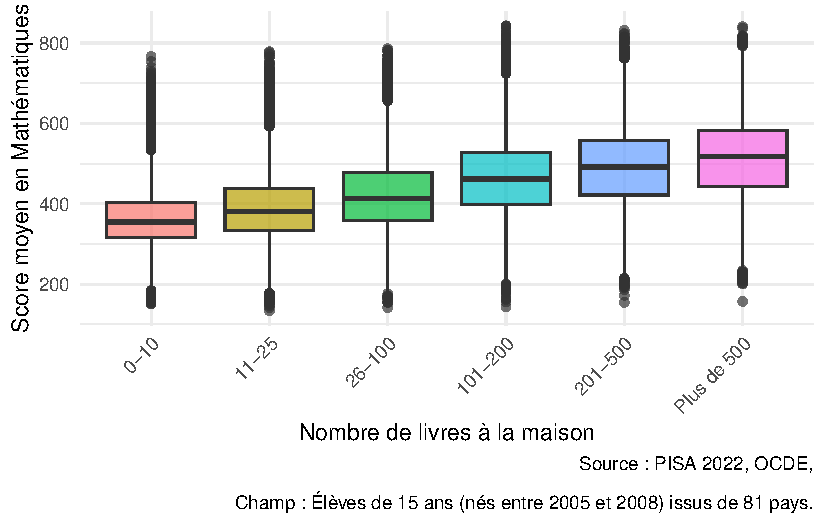
\includegraphics[keepaspectratio]{note_etape_files/figure-pdf/fig-livres-1.pdf}}

}

\caption{\label{fig-livres}Scores en mathématiques selon les ressources
au domicile}

\end{figure}%

La lecture de cette boîte à moustaches (boxplot) révèle un gradient
socio-scolaire extrêmement marqué. L'axe des abscisses, qui catégorise
le nombre de livres au domicile (un indicateur classique du capital
matériel et culturel), montre une corrélation positive évidente avec la
distribution des scores en mathématiques (axe des ordonnées).

-Une progression linéaire des médianes : On observe que la médiane des
scores s'élève systématiquement à chaque palier de ressources. Les
élèves déclarant posséder ``0 à 10 livres'' présentent la médiane la
plus faible (généralement située dans le bas de l'échelle PISA), tandis
que ceux vivant dans un foyer avec ``Plus de 500 livres'' affichent la
médiane la plus haute.

-La dispersion des scores : La position des ``boîtes'' (qui concentrent
50 \% des effectifs centraux de chaque catégorie) est également
révélatrice. On remarque souvent que le 1er quartile (le bas de la
boîte) des élèves très favorisés (plus de 200 livres) est supérieur à la
médiane, voire au 3ème quartile, des élèves les plus démunis (0-10
livres).

Pour confirmer ces observations visuelles, nous croisons une variable
quantitative continue (le score en maths) avec nos variables
qualitatives à l'aide de tests d'Analyse de Variance (ANOVA).

\begin{verbatim}
                Df    Sum Sq   Mean Sq F value Pr(>F)    
Nb_Livres        5 8.796e+08 175917672   23256 <2e-16 ***
Residuals   442117 3.344e+09      7565                   
---
Signif. codes:  0 '***' 0.001 '**' 0.01 '*' 0.05 '.' 0.1 ' ' 1
17211 observations effacées parce que manquantes
\end{verbatim}

\begin{verbatim}
Eta-carré du nombre de livres : 0.2082 
\end{verbatim}

Le test d'analyse de variance (ANOVA) révèle un Êta-carré de 0.2082.
D'un point de vue statistique, ce résultat indique que près de 21 \% des
écarts de performance en mathématiques entre les élèves sont expliqués
par le seul indicateur du nombre de livres au domicile.

Dans le champ des sciences sociales et de l'éducation, il s'agit d'une
taille d'effet considérée comme très forte. Ce chiffre
exceptionnellement élevé démontre la puissance du déterminisme
socio-culturel : l'accès aux ressources matérielles et culturelles dans
l'environnement familial n'est pas un simple facteur d'influence, mais
bien un prédicteur majeur de la réussite scolaire.

Le second graphique porte sur une condition d'existence fondamentale :
ne pas avoir faim.

\begin{figure}

\centering{

\pandocbounded{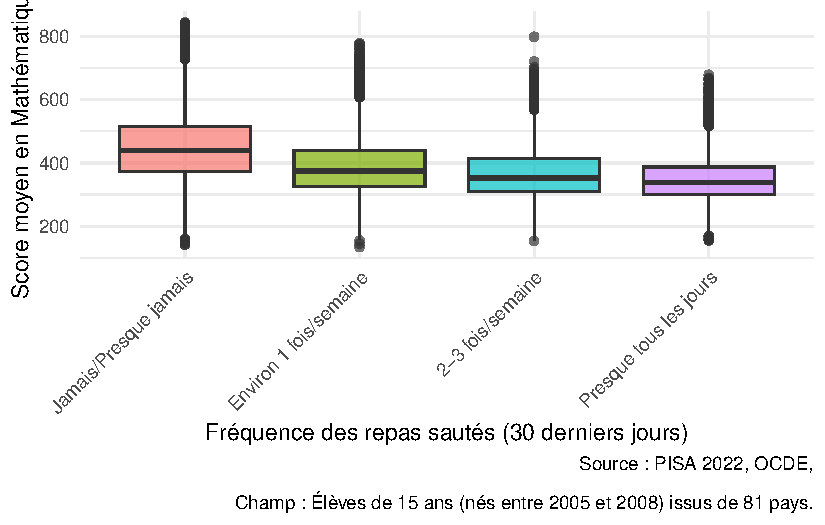
\includegraphics[keepaspectratio]{note_etape_files/figure-pdf/fig-faim-1.pdf}}

}

\caption{\label{fig-faim}Scores en mathématiques selon la précarité
alimentaire}

\end{figure}%

Ce graphique aborde la précarité sous son angle le plus primaire :
l'incapacité à se nourrir correctement par manque d'argent. La
visualisation met en évidence une rupture franche dans les trajectoires
scolaires dès l'apparition de ce facteur.

L'effet ``seuil'' de la précarité : Le groupe majoritaire des élèves qui
ne sautent ``Jamais / Presque jamais'' de repas affiche une distribution
des scores tirée vers le haut, avec une médiane nettement supérieure aux
autres groupes.

Le décrochage des performances : Dès que l'élève bascule dans
l'insécurité alimentaire, même de façon occasionnelle (``Environ 1 fois
par semaine''), on observe un affaissement brutal de la boîte à
moustaches. La médiane chute significativement, et la moustache
inférieure s'étire vers les scores les plus bas de l'évaluation PISA.
Les catégories d'insécurité sévère (``2-3 fois par semaine'' et
``Presque tous les jours'') confirment ce maintien à un niveau de
performance très faible.

\begin{verbatim}
                   Df    Sum Sq  Mean Sq F value Pr(>F)    
Faim_Frequence      3 2.144e+08 71461067    7772 <2e-16 ***
Residuals      435419 4.003e+09     9194                   
---
Signif. codes:  0 '***' 0.001 '**' 0.01 '*' 0.05 '.' 0.1 ' ' 1
23911 observations effacées parce que manquantes
\end{verbatim}

\begin{verbatim}
Eta-carré de l'insécurité alimentaire : 0.0508 
\end{verbatim}

Le test d'analyse de variance (ANOVA) indique un Êta-carré de 0.0508.
Cela signifie qu'à elle seule, la fréquence de l'insécurité alimentaire
explique un peu plus de 5 \% (5,08 \%) de la variance globale des scores
en mathématiques.

En sciences sociales, une valeur autour de 0.06 est considérée comme un
effet de taille moyenne. Cependant, il faut remettre ce chiffre dans son
contexte : la réussite en mathématiques est un processus cognitif
complexe, influencé par des dizaines de facteurs (pédagogie, soutien
familial, temps de travail, etc.). Qu'une seule variable, purement
physiologique et mesurant un besoin primaire, parvienne à dicter 5 \% de
la note finale est un résultat particulièrement fort.

Contrairement au `nombre de livres' qui agit comme un indicateur global
englobant le capital économique et culturel de toute la famille
(expliquant \textasciitilde20 \% de la variance), l'insécurité
alimentaire cible spécifiquement la frange la plus précaire des élèves.
Ce résultat de 5 \% prouve statistiquement ce que la pyramide de Maslow
théorise : l'incapacité à combler un besoin physiologique fondamental
(se nourrir) dresse une barrière immédiate et mesurable à la
disponibilité cognitive (le focus) nécessaire pour les apprentissages
scolaires.

Une immense majorité des élèves n'a pas faim . La variable ne discrimine
donc ``que'' le bas du spectre social. Expliquer 5 \% de la variance
totale de toute une population avec un phénomène qui ne touche qu'une
minorité d'élèves est la preuve absolue que l'impact sur ces élèves
spécifiques est dévastateur.

L'analyse croisée des données de l'enquête PISA 2022 confirme de manière
univoque notre hypothèse de départ : l'accès aux ressources matérielles
reste un enjeu prédominant, voire déterminant, du succès scolaire en
mathématiques.

Au fil de cette partie, nous avons pu mettre en lumière que l'échec ou
la réussite d'un élève ne relève pas de ses seules capacités cognitives
innées, mais est lourdement dicté par son environnement extérieur, selon
deux échelles distinctes :

\textbf{1. Le déterminisme socio-culturel structurel (Le capital
matériel)} L'étude du nombre de livres au domicile a démontré que le
capital culturel et économique de la famille structure massivement les
trajectoires d'apprentissage. Avec près de 21 \% de la variance des
scores en mathématiques expliquée par ce seul indicateur, nos résultats
corroborent les théories de la reproduction sociale. L'école peine à
compenser ces inégalités de départ : les élèves évoluant dans un
environnement riche en ressources (matérielles, espace de travail, accès
à la culture) disposent d'un avantage comparatif écrasant qui se traduit
directement dans leurs résultats.

\textbf{2. Le prérequis physiologique incontournable (Les conditions
d'existence)} Plus alarmant encore, l'analyse de l'insécurité
alimentaire a révélé l'impact foudroyant de la précarité primaire. Bien
qu'elle ne touche qu'une minorité d'élèves, elle explique à elle seule
plus de 5 \% de la variance globale des scores.

\section{B. La transmission familiale du capital scientifique explique
les résultats en
maths}\label{b.-la-transmission-familiale-du-capital-scientifique-explique-les-ruxe9sultats-en-maths}

Les résultats suggèrent que les élèves issus de familles où les parents
possèdent un niveau d'études supérieur obtiennent, en moyenne, de
meilleurs scores en mathématiques. Ce phénomène illustre le poids du
bagage académique familial dans la réussite scolaire.

\begin{figure*}[H]

\pandocbounded{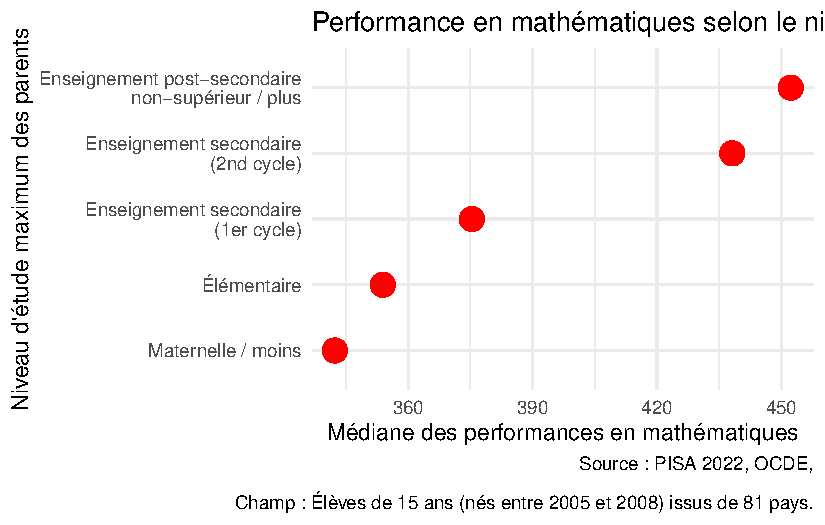
\includegraphics[keepaspectratio]{note_etape_files/figure-pdf/unnamed-chunk-4-1.pdf}}

\end{figure*}

Pour dépasser la simple observation visuelle et confirmer cette
tendance, nous avons réalisé une analyse de la variance (test ANOVA)
accompagnée du calcul de l'Eta-carré (\(\eta^2\)). L'Eta-carré permet de
mesurer la taille de l'effet, c'est-à-dire la proportion de la variance
des scores en mathématiques qui est directement expliquée par le niveau
d'études des parents.

P-value :

\begin{verbatim}
[1] 0
\end{verbatim}

Taille de l'effet (Eta-carré) :

\begin{verbatim}
                                  eta.sq eta.sq.part
as.factor(niveau_famille_max) 0.07774154  0.07774154
\end{verbatim}

\subsubsection{Interprétation}\label{interpruxe9tation}

La p-value étant largement inférieure au seuil de 0,05, nous pouvons
affirmer que la différence de niveau en mathématiques selon le diplôme
des parents est statistiquement significative.

Par ailleurs, l'Eta-carré nous indique que le niveau d'études parental
explique environ 7,1 \% de la variance des résultats en mathématiques.
Si ce pourcentage peut sembler numériquement modeste, il représente en
réalité un effet notable en sciences sociales. Il confirme l'influence
décisive du bagage académique familial, tout en rappelant logiquement
que la réussite de l'élève dépend d'une multitude d'autres facteurs
(environnement scolaire, pédagogie, travail personnel, etc.).

\subsection{Première conclusion et hypothèse du capital
culturel}\label{premiuxe8re-conclusion-et-hypothuxe8se-du-capital-culturel}

Le parcours académique des parents a donc un impact avéré sur le niveau
en mathématiques des enfants. Cela peut s'expliquer par une transmission
informelle des savoirs, un accompagnement scolaire plus aisé, ou encore
une valorisation de la réussite scolaire davantage intériorisée par la
famille.

Pour approfondir cette dynamique, nous pouvons formuler l'hypothèse que
ce niveau d'études se matérialise aussi par un environnement culturel
plus riche au domicile. Dans la continuité des théories sur la
reproduction sociale, le diplôme (qui correspond au capital culturel
institutionnalisé) s'accompagne souvent de ressources intellectuelles et
matérielles favorisant l'apprentissage (le capital culturel objectivé).
Dans la partie précédente, nous avons d'ailleurs montré que les
ressources matérielles étaient liées à la réussite en mathématiques.

Croisons maintenant le niveau d'études des parents avec un indicateur
classique de ce capital culturel : le nombre de livres présents au
domicile.

\begin{figure*}[H]

\pandocbounded{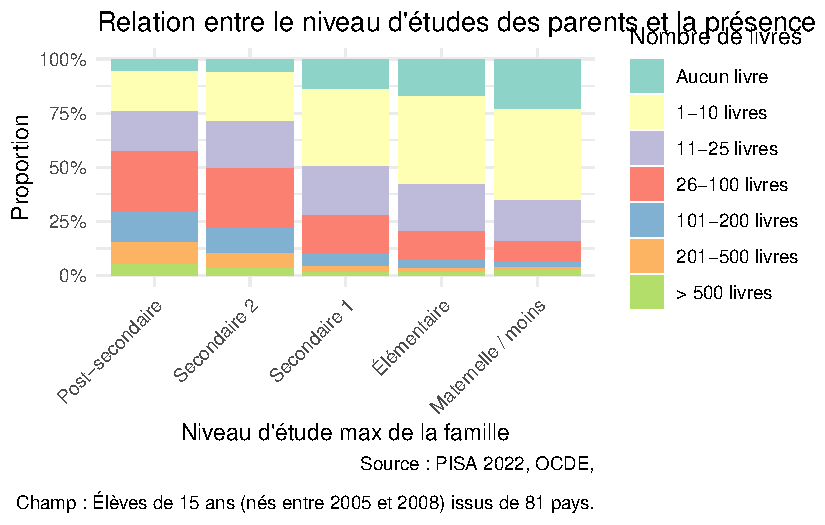
\includegraphics[keepaspectratio]{note_etape_files/figure-pdf/unnamed-chunk-8-1.pdf}}

\end{figure*}

Graphiquement, on observe une corrélation très claire entre le nombre de
livres à la maison et le diplôme des parents : plus le diplôme est
élevé, plus la proportion de familles disposant d'une grande
bibliothèque augmente.

Nous le vérifions avec un test d'indépendance du Chi-deux (Khi2) :

\begin{verbatim}

    Pearson's Chi-squared test

data:  tableau
X-squared = 39123, df = 24, p-value < 2.2e-16
\end{verbatim}

\subsubsection{Interprétation}\label{interpruxe9tation-1}

La p-value étant extrêmement proche de zéro (largement inférieure à
0,05), nous rejetons l'hypothèse d'indépendance. Les deux variables sont
très fortement dépendantes. Le niveau d'études maximum des parents est
donc intimement corrélé à la mise en place d'un environnement culturel
et matériel propice à l'apprentissage (ici, l'accès aux livres).

Il est alors intéressant d'isoler le facteur de la richesse : à niveau
de vie (ou richesse matérielle) égal, les enfants dont les parents sont
les plus diplômés réussissent-ils toujours mieux en mathématiques ?

\begin{figure*}[H]

\pandocbounded{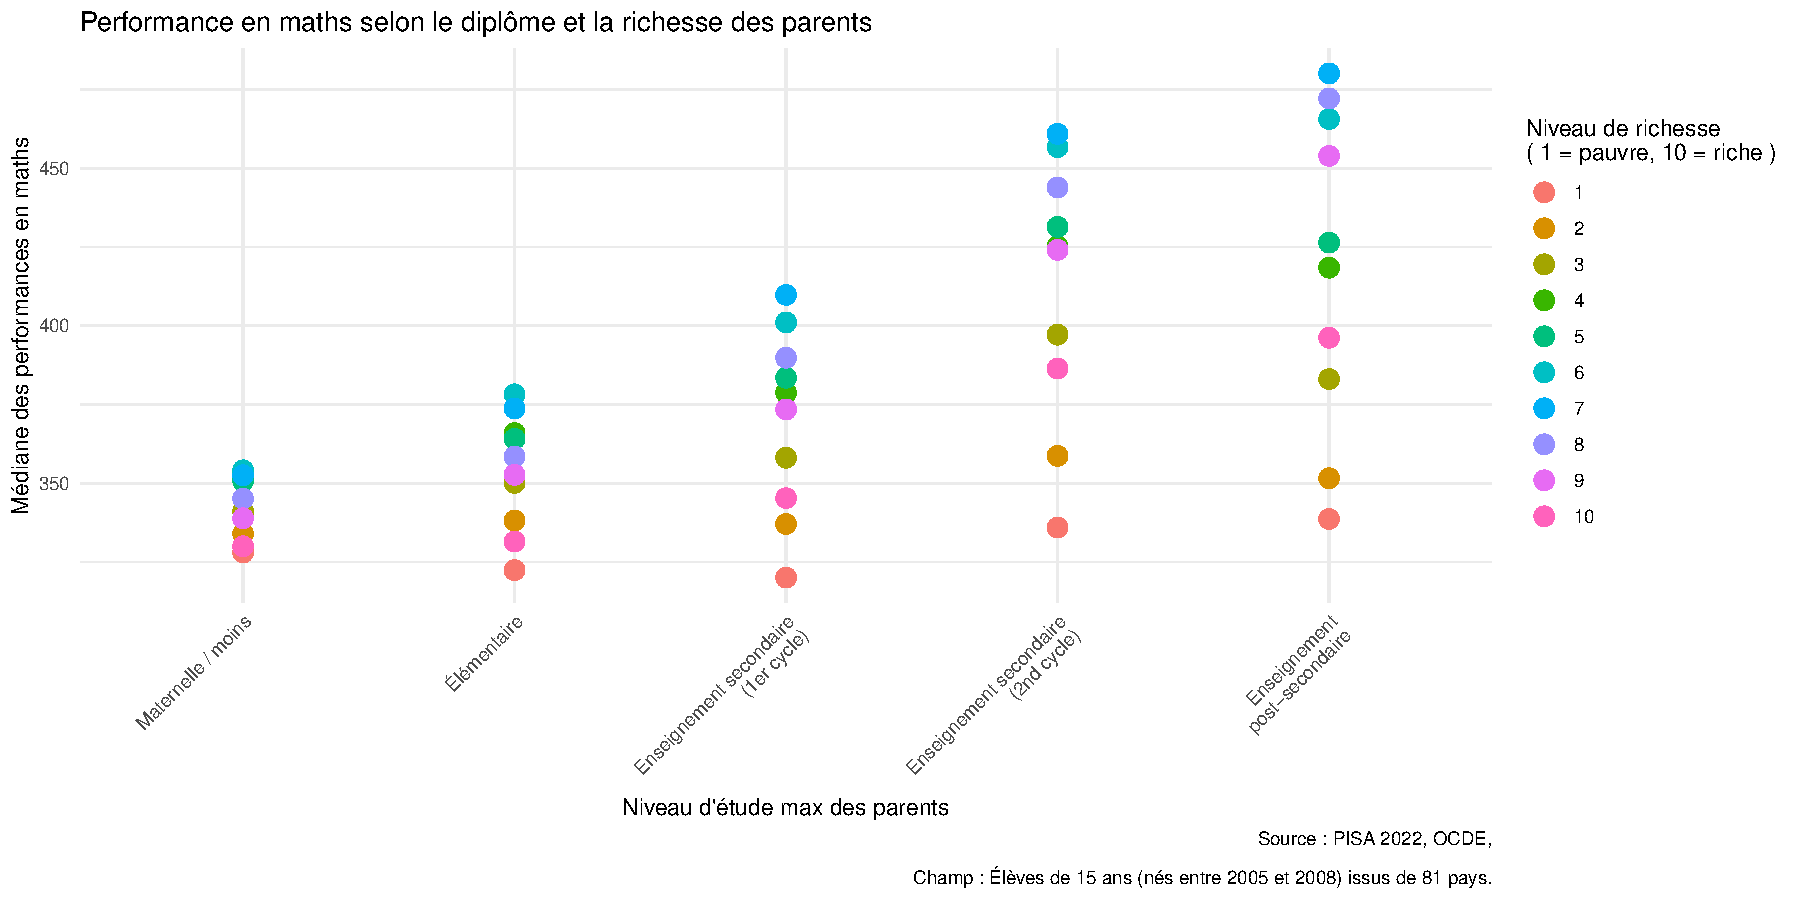
\includegraphics[keepaspectratio]{note_etape_files/figure-pdf/unnamed-chunk-10-1.pdf}}

\end{figure*}

Ce graphique est révélateur : en suivant n'importe quelle courbe de
niveau de richesse, on observe toujours une tendance ascendante vers les
plus hauts diplômes. Cela démontre que, même à niveau de vie égal, le
niveau d'études des parents conserve un impact positif et distinct sur
la performance en mathématiques de l'enfant. L'héritage intellectuel et
scientifique ne se résume donc pas au seul confort économique.

\chapter{II) L'élève : une personnalité, un caractère et une pensée qui
assure un niveau
mathématique}\label{ii-luxe9luxe8ve-une-personnalituxe9-un-caractuxe8re-et-une-pensuxe9e-qui-assure-un-niveau-mathuxe9matique}

L'environnement et les différents ``capital'' ont ainsi une réelle
corrélation avec la performance des élèves et nous avons solidement pu
assurer le lien de causalité.\\
Dans l'optique de décrire des profils plus complets des élèves, Nous
allons chercher des paramètres psychologiques, psychosociaux, plus
centrés sur l'élève lui-même et son état d'esprit.

\section{A. Le ``self-made'' student ? Une analyse psychosociale de la
prophétie
auto-réalisatrice}\label{a.-le-self-made-student-une-analyse-psychosociale-de-la-prophuxe9tie-auto-ruxe9alisatrice}

D'après Chavez (\citeproc{ref-chavez25}{Chavez 2025}), il existe une
``prophétie autoréalisatrice'' : La croyance en notre réussite nous
conduit à celle-ci plus facilement. Dans notre cas, les dispositions
psychologiques des élèves joueraient sur la performance en
mathématiques. C'est ce que nous allons analyser dans cette partie.

Notre première variable d'intérêt est celle qui évalue la volonté des
élèves à ``bien vouloir faire en cours de maths''

Comme le montre le graphique suivant, on distingue une corrélation
nette. Les élèves souhaitant bien faire pendant les cours de maths ont
globalement un score mathématique plus élevé.

\pandocbounded{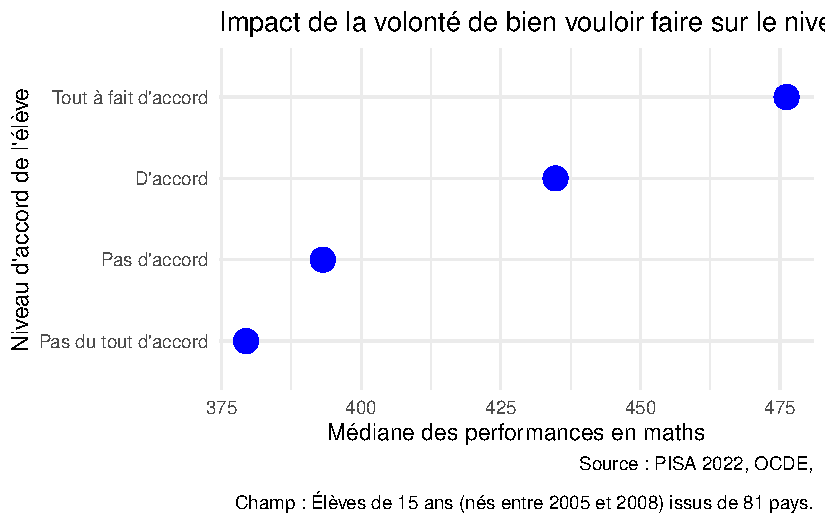
\includegraphics[keepaspectratio]{note_etape_files/figure-pdf/unnamed-chunk-12-1.pdf}}

\begin{verbatim}
La p-value est d'environ : 0 
\end{verbatim}

\begin{verbatim}
Le rapport de corrélation (Eta-carré) est : 0.07924658 
\end{verbatim}

Pour mieux cerner l'impact de cet engagment pendant les cours de
mathématiques, on peut regarder la distribution suivante :

\pandocbounded{\includegraphics[keepaspectratio]{note_etape_files/figure-pdf/unnamed-chunk-14-1.pdf}}

On confirme l'analyse du premier graphe mais ramené à tous les élèves,
elle semble moins importante. On retrouve en effet nombre d'élève dont
la volonté de bien faire est élevé mais dont les résultats sont bas. En
somme, la volonté est effectivement liée mais il convient de chercher
plus loin pour trouver des relations de causalité. Nous nous
intéresserons donc de la même manière à d'autres variables liées à la
confiance.

La réponse à la question ``les mathématiques sont faciles pour moi''
peut être intéressante. Elle mesure la confiance dans la matière. On
s'attend en premier lieu à ce que les étudiants trouvant les
mathématiques faciles soient effectivement bon. La corrélation est
validée par la p-value mais le rapport de corrélation, de seulement 0.05
montre qu'il y a plus à étudier.

\begin{verbatim}
Variable : ST268Q04JA (Aisance)
\end{verbatim}

\begin{verbatim}
- p-value : < 2.22e-16 
\end{verbatim}

\begin{verbatim}
- Rapport de corrélation (Eta2) : 0.0529 
\end{verbatim}

\pandocbounded{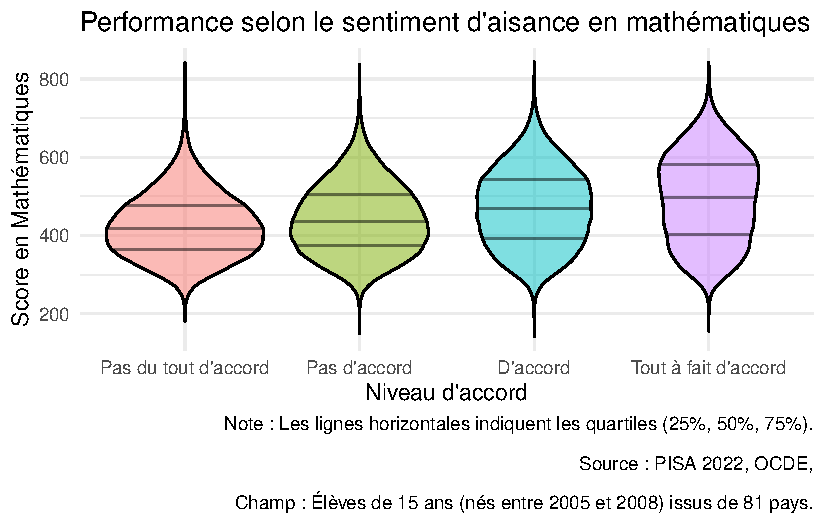
\includegraphics[keepaspectratio]{note_etape_files/figure-pdf/unnamed-chunk-15-1.pdf}}

L'analyse des violin plot nous révèle qu'un grand nombre d'élève sont
confiant en leur performance mais en réalité obtiennent des résultats
plutôt moyens. {[}ajouter un trait pour la médiane de tous les
élèves{]}. La tendances globale attendue est quand même confirmée.

À l'inverse, on peut étudier le contrepied de la confiance à travers
l'anxiété des élèves lorsqu'il résolvent des problèmes mathématiques.
Encore une fois, une corrélation est observée.

\begin{verbatim}
Variable : ST292Q03JA (Anxiété)
\end{verbatim}

\begin{verbatim}
- p-value : < 2.22e-16 
\end{verbatim}

\begin{verbatim}
- Rapport de corrélation (Eta2) : 0.0876 
\end{verbatim}

\pandocbounded{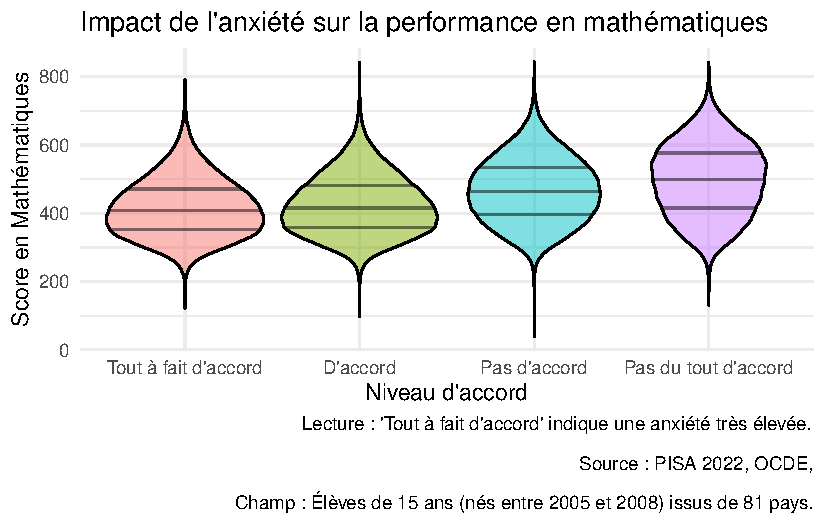
\includegraphics[keepaspectratio]{note_etape_files/figure-pdf/unnamed-chunk-16-1.pdf}}

Mais surprenament, l'intensité de la corrélation est plus grande que les
paramètres précédents. L'analyse montre cependant bien que plus un élève
est anxieux dans la résolution de problèmes, moins il est bon en
mathématiques.

Nous pouvons émincer ce paramètre grâce aux différentes questions qui
ciblent la confiance à résoudre un certain type de problème
mathématiques.

\pandocbounded{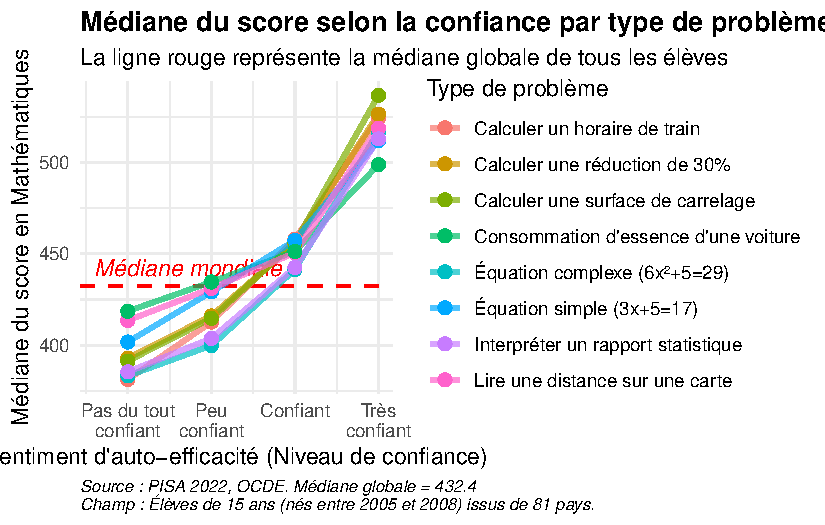
\includegraphics[keepaspectratio]{note_etape_files/figure-pdf/unnamed-chunk-17-1.pdf}}

Les résultats sont ceux attendus : Plus les élèves sont confiants,
meilleurs sont leur score en mathématique.

En somme, la corrélation entre la confiance de réussite est bien
apparente sur tous les aspects considérés. Cependant il est assz
difficile d'établir une causalité qui validerait la prophétie
autoréalisatrice. Les données montrent surtout le sens inverse, logique
: meilleur on est, plus on se sent confiant.

Pour chercher des réelles causalité d'une confiance qui pourrait amener
à performer il faut étudier la psychologie et la manière de penser des
élèves et ce dans la vie de tous les jours.

\section{B. Une vision psychologique et personnelle adaptée pour un
meilleur niveau
?}\label{b.-une-vision-psychologique-et-personnelle-adaptuxe9e-pour-un-meilleur-niveau}

Dans cette partie nous chercherons à voir si certains états d'esprit,
certaines manières de penser ont un lien avec les performances
mathématiques. En particulier, est-ce que la perception des capacités
des élèves pourrait être un facteur expliquant un bon niveau en
mathématiques

Pour commencer nous choisissons la variable qui cherche à savoir si les
élèves abandonnent facilement.

\pandocbounded{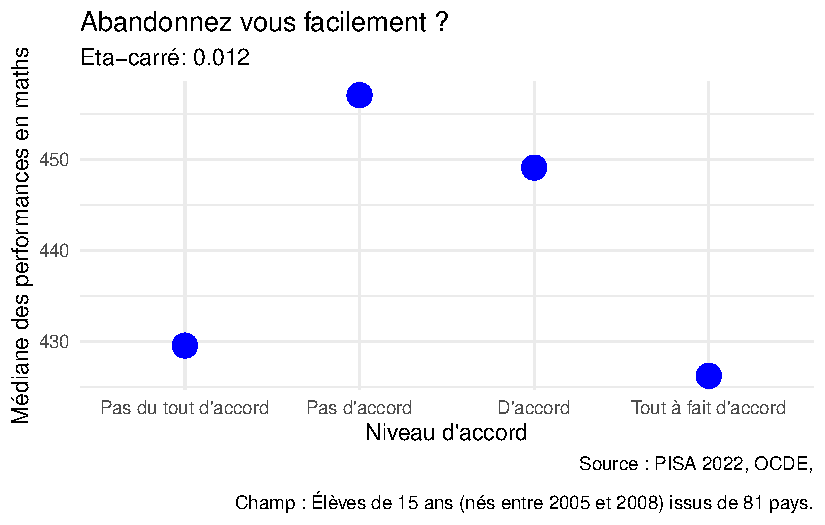
\includegraphics[keepaspectratio]{note_etape_files/figure-pdf/unnamed-chunk-18-1.pdf}}

On observe aucune corrélation. Il en va de même pour les autres
variables liées à la persévérance. Nous n'avons pas grand chose à en
tirer. Essayons une variable liée au stress.

\pandocbounded{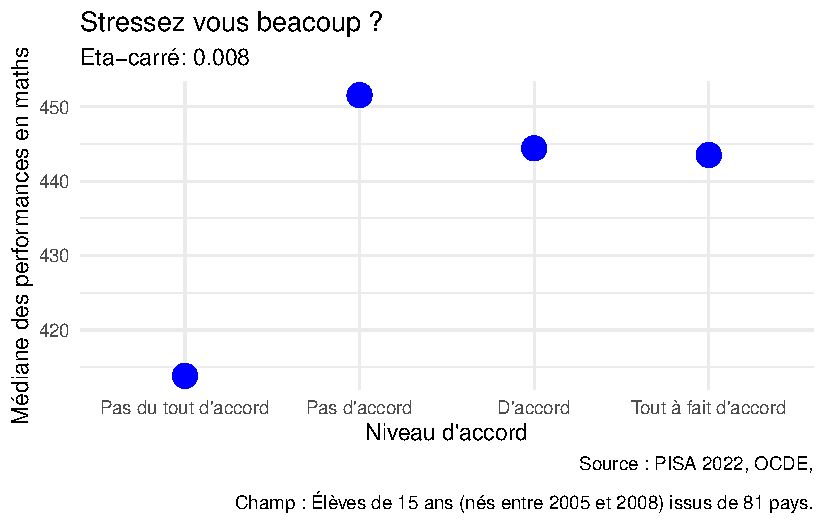
\includegraphics[keepaspectratio]{note_etape_files/figure-pdf/unnamed-chunk-19-1.pdf}}

Malheureusement il est assez difficile de trouver des corrélations
directes à partir de caractéristiques spécifiques. Des points
psychologiques précis ne nous informe pas sur une potentielle
performance mathématiques. Nous chercherons alors à généraliser des
profils en combinant un plus garnd nombre de variables.

La première partie a établi que les performances en mathématiques
s'inscrivent dans un gradient social marqué : le capital économique et
culturel des familles structure fortement la probabilité d'appartenir au
groupe des élèves les plus performants. La seconde partie a toutefois
nuancé cette lecture en mettant en évidence le rôle autonome des
dispositions psychosociales --- auto-efficacité, rapport aux
mathématiques, anxiété --- suggérant qu'une part de la réussite relève
de mécanismes d'appropriation individuelle. Ce résultat peut apparaître,
à première vue, en tension avec l'idée d'un déterminisme socio-familial
prépondérant.

Dès lors, l'enjeu n'est plus d'opposer structure et agentivité, mais
d'examiner leur articulation. La question devient : comment ces
dimensions s'ordonnent-elles conjointement dans l'espace des élèves ?
L'analyse multivariée conduite sur les données de l'enquête PISA 2022
vise précisément à répondre à cette interrogation en appréhendant
simultanément ressources familiales et dispositions individuelles.

L'hypothèse retenue est que l'excellence en mathématiques correspond à
une position spécifique dans un espace structuré conjointement par les
ressources socio-familiales et les dispositions psychosociales. Cet
espace mettrait en évidence un principe de cumul des avantages ---
sociaux et subjectifs --- tout en révélant l'existence de trajectoires
différenciées vers la performance. Il ne s'agit donc ni d'additionner
des effets séparés, ni de hiérarchiser a priori les facteurs, mais
d'identifier la configuration empirique au sein de laquelle s'inscrit le
profil des élèves performants.

\chapter{III) La performance en mathématiques résulte d'une position
spécifique dans un espace structuré par les ressources familiales et les
dispositions
psychosociales}\label{iii-la-performance-en-mathuxe9matiques-ruxe9sulte-dune-position-spuxe9cifique-dans-un-espace-structuruxe9-par-les-ressources-familiales-et-les-dispositions-psychosociales}

\section{A) Les élèves performants cumulent des ressources sociales et
des dispositions psychologiques
favorables}\label{a-les-uxe9luxe8ves-performants-cumulent-des-ressources-sociales-et-des-dispositions-psychologiques-favorables}

\subsection{i) Le cumul des capitaux et des dispositions accroît
fortement la probabilité d'appartenir au groupe
performant}\label{i-le-cumul-des-capitaux-et-des-dispositions-accrouxeet-fortement-la-probabilituxe9-dappartenir-au-groupe-performant}

La thèse selon laquelle le cumul des ressources familiales et des
dispositions personnelles augmente la probabilité d'être un élève
performant en mathématiques s'appuie sur des observations empiriques
solides. Les résultats précédents montrent que les élèves dont les
familles disposent d'un niveau d'éducation élevé et de biens culturels
et matériels tendent à obtenir de meilleurs scores. Parallèlement, la
motivation, la confiance en soi et l'intérêt pour les mathématiques
jouent un rôle important dans la réussite individuelle. Cela suggère que
la performance ne peut pas être expliquée par une seule dimension : elle
résulte de l'interaction entre l'environnement familial et les
ressources personnelles de l'élève.

Pour tester cette hypothèse, il est pertinent de recourir à une analyse
en composantes principales (ACP). Cette méthode permet de résumer un
grand nombre de variables corrélées en quelques axes principaux, qui
représentent les dimensions centrales de variation dans les données. En
projetant les élèves dans cet espace, il devient possible de vérifier si
les meilleurs scores correspondent à une combinaison élevée de
ressources familiales et de dispositions individuelles, et ainsi de
mettre en évidence le principe de cumul des avantages. L'ACP fournit
donc un cadre clair pour identifier les facteurs principaux qui
expliquent la performance et pour situer les élèves performants dans
l'ensemble de l'échantillon.

\pandocbounded{\includegraphics[keepaspectratio]{note_etape_files/figure-pdf/unnamed-chunk-21-1.pdf}}

\pandocbounded{\includegraphics[keepaspectratio]{note_etape_files/figure-pdf/unnamed-chunk-21-2.pdf}}

L'ACP réalisée se concentre dans un premier temps sur les variables
relatives aux ressources familiales (niveau d'études et diplômes des
parents, biens matériels, statut social subjectif) et aux dispositions
psychologiques des élèves (motivation, intérêt, confiance et anxiété en
mathématiques). Ce choix permet de mettre en évidence l'interaction
directe entre environnement socio-familial et traits individuels, en
accord avec l'hypothèse selon laquelle le cumul de ces facteurs favorise
la performance.

L'analyse montre que les deux premières composantes expliquent une part
importante de la variance et reflètent respectivement un gradient de
capital familial cumulé et un gradient de dispositions personnelles. Les
flèches des variables indiquent clairement quelles dimensions
contribuent le plus à chaque axe, et des directions opposées signalent
des effets contrastés entre certaines ressources ou attitudes.

Parmi les limites, il convient de noter que certaines variables
initialement prévues ont été exclues en raison de valeurs manquantes ou
de faible variance, et que l'ACP synthétise l'information sans restituer
la totalité des nuances individuelles. Malgré ces contraintes,
l'approche reste pertinente pour identifier les tendances globales et
caractériser la position des élèves performants dans l'espace
socio-psychologique.

Le biplot permet de visualiser simultanément la position des élèves et
la contribution des variables aux axes, offrant une lecture intégrée de
l'ACP et mettant en évidence à la fois les tendances principales et les
limites liées à la synthèse des données.

\pandocbounded{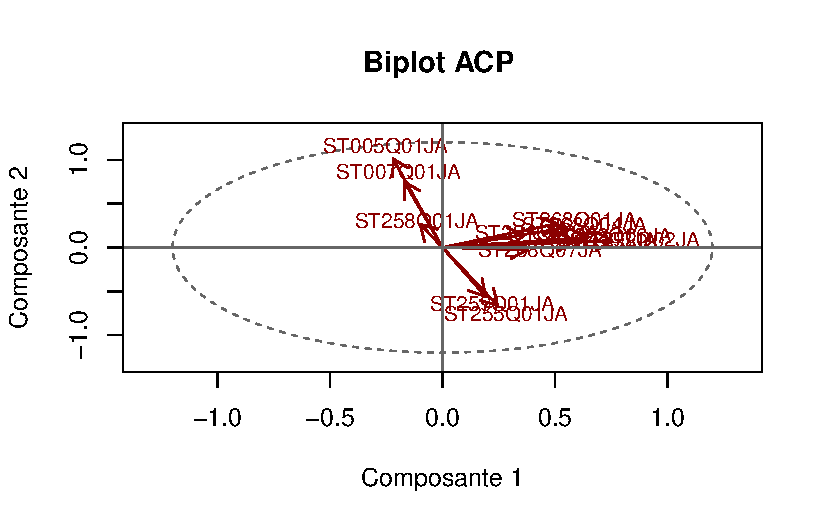
\includegraphics[keepaspectratio]{note_etape_files/figure-pdf/unnamed-chunk-22-1.pdf}}

Sans surprise, on constate que des conditions de vie comme la faim
(ST258Q01JA) sont négativement corrélé au indicateur d'un statut social
favorisé (ST259Q01JA, nombre de livre à la maison: ST255Q01JA).
L'orthogonalité relative entre le groupe des variables psychologiques (à
droite) et celle de la famille indique une certaine indépendance entre
ces deux catégories de facteurs. On peut donc dans un premier temps
supposer que l'une ne cause pas tant l'autre. En revanche ce biplot
n'indique pas clairement la situation des élèves performants.

\subsection{ii) Les élèves performants occupent une zone spécifique de
l'espace
socio-psychologique}\label{ii-les-uxe9luxe8ves-performants-occupent-une-zone-spuxe9cifique-de-lespace-socio-psychologique}

La thèse selon laquelle les élèves performants occupent une zone
spécifique de l'espace socio-psychologique repose sur l'idée que la
réussite en mathématiques résulte de la combinaison de ressources
familiales et de dispositions personnelles favorables. Les observations
précédentes montrent que ces deux dimensions interagissent : certains
élèves peuvent compenser un capital familial modeste par une forte
motivation et confiance en mathématiques, tandis que d'autres
bénéficient de l'effet cumulatif de ressources élevées et de
dispositions favorables.

Pour vérifier cette hypothèse, les élèves du top 10 \% en mathématiques
se projettent sur l'espace factoriel déjà construit par l'ACP. Cette
projection permet d'identifier la zone où se concentrent les meilleurs
scores et de visualiser comment le cumul des facteurs familiaux et
psychologiques se traduit concrètement dans la performance. L'approche
offre une lecture intégrée, mettant en évidence les profils combinant
capital familial et dispositions personnelles élevées.

Il convient de rappeler que cette projection ne modifie pas l'ACP
elle-même et que la synthèse multidimensionnelle masque certaines
nuances individuelles. Néanmoins, elle permet de situer clairement les
élèves performants dans l'espace socio-psychologique et justifie la
construction du biplot suivant, qui met en lumière la zone de haute
probabilité de performance.

\pandocbounded{\includegraphics[keepaspectratio]{note_etape_files/figure-pdf/unnamed-chunk-23-1.pdf}}

\begin{verbatim}
                                                                   Quadrant
Capital élevé / Dispositions modérées Capital élevé / Dispositions modérées
Cumul élevé                                                     Cumul élevé
Cumul faible                                                   Cumul faible
Dispositions fortes / Capital faible   Dispositions fortes / Capital faible
                                      Part_performants
Capital élevé / Dispositions modérées            0.198
Cumul élevé                                      0.112
Cumul faible                                     0.053
Dispositions fortes / Capital faible             0.019
\end{verbatim}

L'observation des élèves du top 10 \% en mathématiques confirme dans
l'ensemble ce que l'on pouvait anticiper : la majorité se situe dans la
zone où le capital familial et les dispositions personnelles sont
élevés. Cependant, quelques exceptions apparaissent, montrant que
certains élèves réussissent malgré un capital familial modeste ou que
d'autres ne performent pas pleinement malgré des ressources favorables.
Ces exceptions conduisent à nuancer l'hypothèse d'un modèle unique de
réussite et à envisager la nécessité d'une typologie des profils.
L'excellence en mathématiques n'est pas monolithique et semble pouvoir
se décliner en plusieurs trajectoires : une voie « héritière »,
combinant fort capital et forte confiance ; une voie « résiliente »,
caractérisée par un capital modeste mais une auto-efficacité élevée ; et
éventuellement une voie « structure compensée », où un capital familial
important coexiste avec des dispositions moyennes. Une classification de
ce type permettrait d'identifier et de caractériser distinctement ces
profils, offrant ainsi un outil plus précis pour comprendre la diversité
des trajectoires vers la performance.

\pagebreak

\chapter{Conclusion}\label{conclusion}

Être riche ça aide

\chapter{Références}\label{pagedesreferences}

Voici la liste de toutes les références bibliographiques utiles à la
rédaction de ce rapport :

\protect\phantomsection\label{refs}
\begin{CSLReferences}{1}{1}
\bibitem[\citeproctext]{ref-chavez25}
Chavez. 2025. {«~titre~»}. \emph{Journal of Evaluation in Education}, nᵒ
1.

\bibitem[\citeproctext]{ref-vanmechelen2019}
Mechelen, Erik van. 2019. \emph{How to Be a Diplomacy Player: A
Philosophy of Face to Face Diplomacy}. Lean Publishing.

\end{CSLReferences}

\chapter{Annexes}\label{pagesdannexes}




\end{document}
